\subsubsection{Description / circuitry}
% Describe the tractive system active light and additional circuitry. Additionally, fill out the table:

The TSAL is a distributed system consisting of the following components:
\begin{itemize}
\item Tractive System Active Light mounted on main hoop
\item TSAL logic \& power circuitry (located in ECU-B; LV only)
\item DC-DC converter to power the TSAL in case of charged TS but unpowered GLVS (located in the ACP; has a HV side and a LV side)
\end{itemize}

\paragraph{Tractive System Active Light}

The TSAL proper is connected with 2 wires. When voltage of 24 V is applied, the TSAL lights up either in green or red color depending on the polarity.

% TODO aktualizovat schema
\begin{figure}[H]
	\centering
	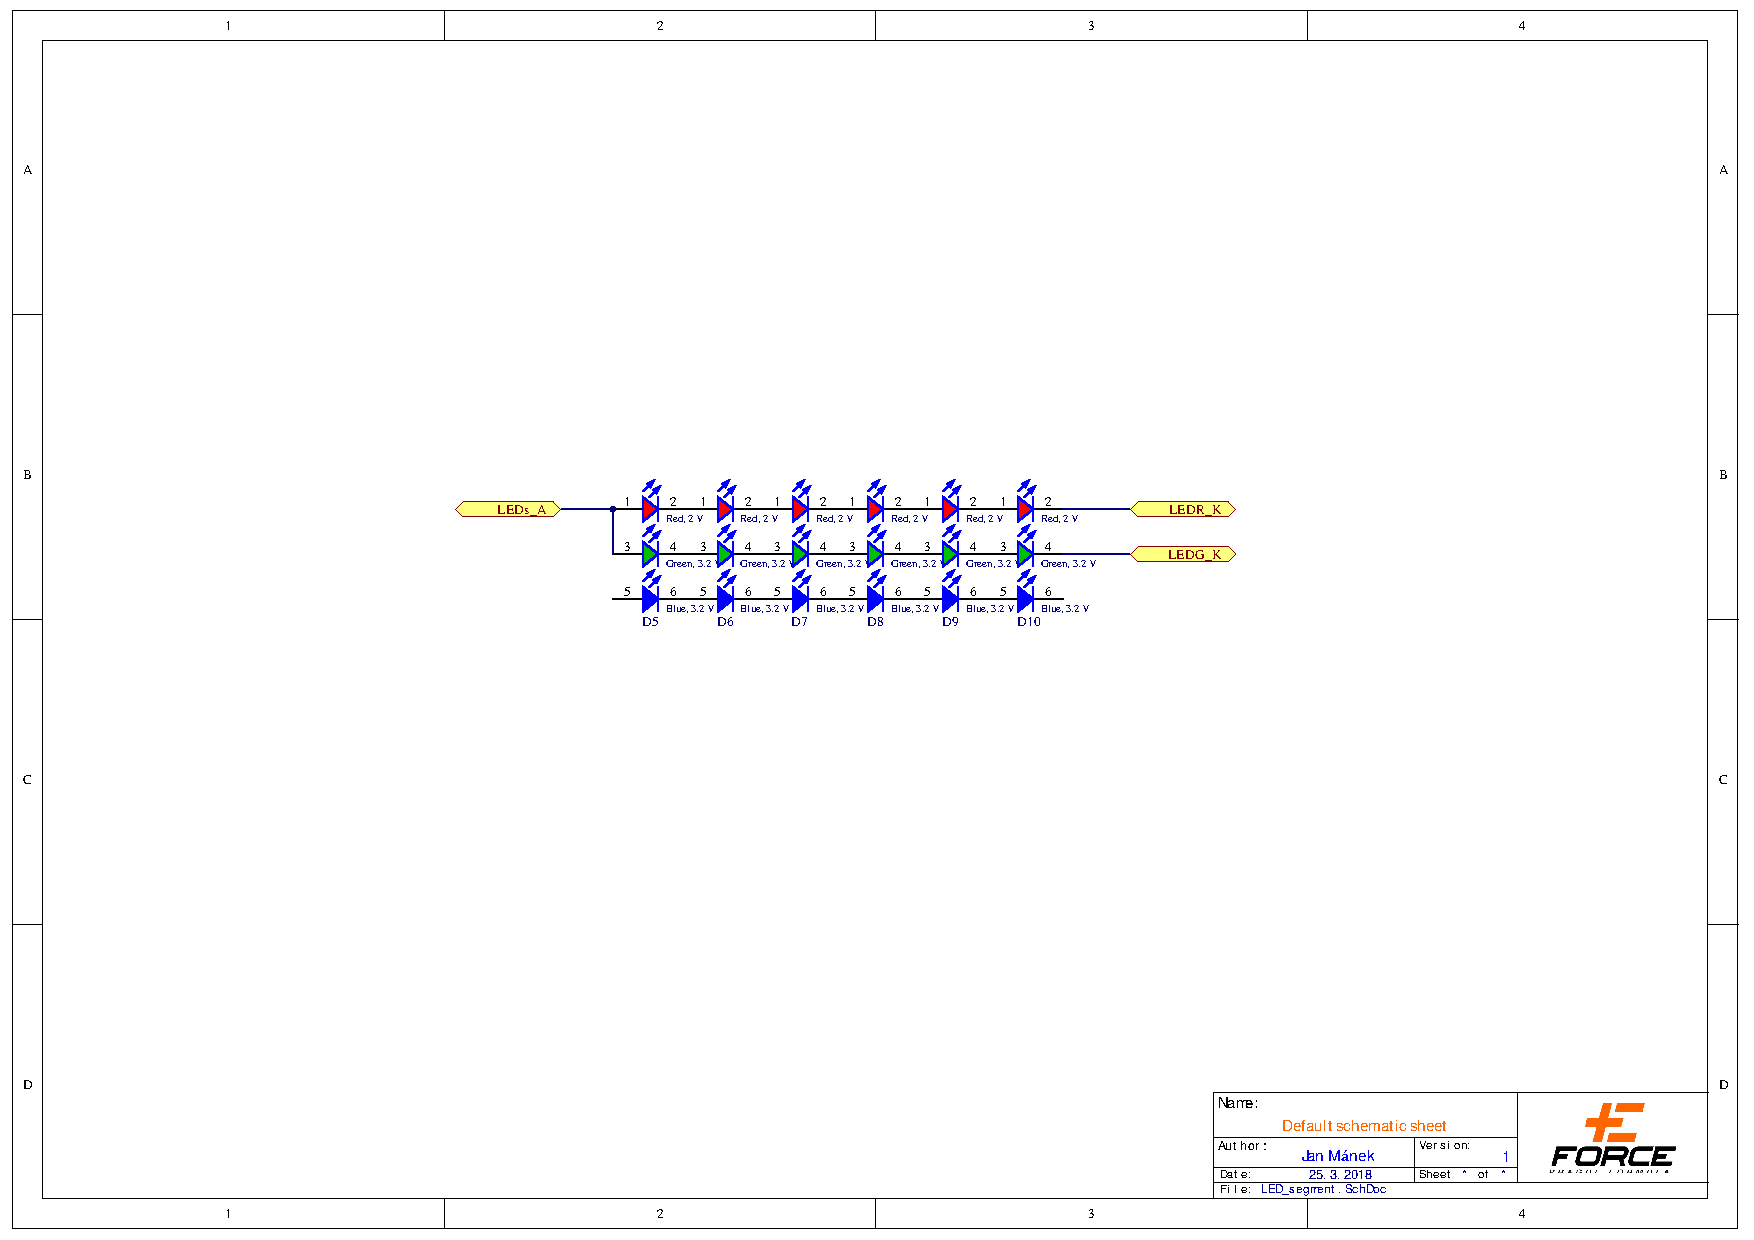
\includegraphics[width=\textwidth,trim={6cm 10cm 6cm 7cm},clip]{./img/TSAL-schematic.pdf}
	\caption{TSAL schematic.}
	\label{fig:TSAL-schematic}
\end{figure}

\begin{table}[H]
	\centering
	\caption{Parameters of the TSAL}
	\begin{tabularx}{\textwidth}{|X|X|}
		\hline
		Supply voltage: & +/- 24VDC \\[\TableSize]
		\hline
		Max. operational current: & 300mA \\[\TableSize]
		\hline
		Lamp type & Bi-color LED \\[\TableSize]
		\hline
		Power consumption: & 7.2 W \\[\TableSize]
		\hline
		Brightness & 124 Lumen (red), 29 Lumen (green) \\[\TableSize]
		\hline
		Frequency: & 3.96Hz \\[\TableSize]
		\hline
		Size (length x height x width): & 128mm x 20mm x 32mm \\[\TableSize]
		\hline
	\end{tabularx}%
	\label{tab:TSAL}%
\end{table}%

\paragraph{TSAL logic \& power circuitry}

To power the TSAL, a voltage of approximately 24 V is needed. This can be supplied either by the GLVS, or by a charged Tractive System by means of an isolated DC-DC converter.

A 5V rail is also generated to control all TSAL-related logic. (\ref{fig:TSAL-ECUB-5V})

\begin{figure}[H]
	\centering
	\includegraphics[width=0.6\textwidth]{./img/TSAL-ECUB-5V.png}
	\caption[Powering of the TSAL]{Powering of the TSAL. GLVS power is denoted \texttt{VCC}.}
	\label{fig:TSAL-ECUB-5V}
\end{figure}

Discrete logic is used for selecting the light colour. (\ref{fig:TSAL-logic})

\begin{figure}[H]
	\centering
	\includegraphics[width=\textwidth]{./img/TSAL-logic.png}
	\caption[TSAL enable logic]{TSAL enable logic. The signals \texttt{TSAL-RED} and \texttt{TSAL-GREEN} are always complementary.}
	\label{fig:TSAL-logic}
\end{figure}

A 555 IC is used to generate the required frequency which is used to modulate the power output. (\ref{fig:TSAL-555})

\begin{figure}[H]
	\centering
	\includegraphics[width=0.6\textwidth]{./img/TSAL-555.png}
	\caption[TSAL frequency generator]{TSAL frequency generator. When a green light is desired (GLVS active, TS not charged), oscillation is suppressed and the output \texttt{TSAL-PWM-IN} is a constant logical '1'.}
	\label{fig:TSAL-555}
\end{figure}

Finally, a H-bridge is used to drive the proper power outputs with switchable polarity. (\ref{fig:TSAL-H-bridge})

\begin{figure}[H]
	\centering
	\includegraphics[width=0.5\textwidth]{./img/TSAL-H-bridge.png}
	\caption{TSAL power H-bridge}
	\label{fig:TSAL-H-bridge}
\end{figure}

\ref{fig:TSAL-logic-table} summarizes operation of the TSAL.

\begin{table}[H]
	\centering
	\caption{TSAL logic table}
	\begin{tabularx}{\textwidth}{|X|X|X|X|X|}
		\hline
		\textbf{Tractive System state} & \textbf{GLVS state} & \textbf{TSAL powered from} & \textbf{TSAL polarity} & \textbf{TSAL waveform} \\
		\hline
		not charged & off & not powered & -- & -- \\
		\hline
		not charged & on & 24V GLVS & negative (green) & Always-on \\
		\hline
		precharging & on & 24V GLVS & positive (red) & Square wave, 3.96Hz, 50\% duty cycle \\
		\hline
		charged & don't care & TS & positive (red) & Square wave, 3.96Hz, 50\% duty cycle \\
		\hline
	\end{tabularx}%
	\label{fig:TSAL-logic-table}
\end{table}%

\paragraph{DC-DC converter}

To ensure that the TSAL continues to operate even after disabling GLVS, the following circuit is used:

% TODO: JSix + Patrik -- vsechno okolo ACP casti TSALu

\begin{figure}[H]
	\centering
	\includegraphics[width=\textwidth]{./img/tsal-hv.jpg}
	\caption{TSAL HV part schematic.}
	\label{fig:TSAL-HV}
\end{figure}

\paragraph{Explanation of TSAL circuit}

TODO TODO JSix Patrik Left top corner of \ref{fig:TSAL-HV} (input marked as HV-Viper) is directly connected to the output HV pins of ACP. The circuit is designed with STM chip „VIPER16HN“. It behaves as normal fly-back, with input voltage range from 50V up to 500V. Output of flyback is used to directly power the TSAL. ACP indication led is powered from primary side of transformer. To ensure correct behaviour, we also measure and compare input voltage (using U12A OAMP as comparator with little hysteresis), to enable output (Q36 \& Q33) only if input voltage is >=60VDC.

\begin{figure}[H]
	\centering
	\includegraphics[width=\textwidth]{./img/tsal-position.jpg}
	\caption{TSAL enable scheme}
	\label{fig:TSAL-enable}
\end{figure}

Function of circuit on \ref{fig:TSAL-enable} is that the TSAL is enabled even when the 60VDC limit is not reached, but the AIR is closed nonetheless. In such state, the TSAL is enabled by signal AIR\_EN. The circuit is powered by MAIN24 power (which is equal to the 24V enabled by GLVMS) or by the TSAL\_ACP-EN power signal from the Viper-TSAL schematic (\ref{fig:TSAL-ACPindicator}) below.

\begin{figure}[H]
	\centering
	\includegraphics[width=\textwidth]{./img/tsal-indicator.jpg}
	\caption{ACP indication LED wiring}
	\label{fig:TSAL-ACPindicator}
\end{figure}

%schema z backu
\subsubsection{Wiring/cables/connectors}
\iffalse Describe wiring, show schematics, describe connectors and cables used and show useful data regarding the wiring.  Include gauge, voltage and temperature rating of wiring used and any fuses or other overcurrent protection used.\fi

LEDs are supplied from ECUB (by Harness\_D by connector D1) by 2-wire low voltage cable (\ref{fig:TSAL-wiring}).

\begin{figure}[H]
	\centering
	\includegraphics[width=\textwidth,]{./img/tsal-wiring.jpg}
	\caption{Wiring TSAL from ECUB}
	\label{fig:TSAL-wiring}
\end{figure}

\subsubsection{Position in car}
%Provide CAD-renderings showing the relevant parts. Mark the parts in the rendering, if necessary.
TSAL is placed under the main roll hoop, see \ref{fig:TSAL-position}

\begin{figure}[H]
	\centering
	\includegraphics[width=\textwidth,trim={3cm 11cm 2cm 1cm},clip]{./img/tsal-position.pdf}
	\caption{TSAL position.}
	\label{fig:TSAL-position}
\end{figure}
